
\chapter{Collections and Comprehensions}

It is usual for data to form collections: employees; customer transactions;
connected clients. When modelling collections of data it is very convenient
to have language structures that make it easy to create, transform
and filter the collections. This chapter describes how such a language
construct can be defined. 

%
\begin{figure}
\begin{center}

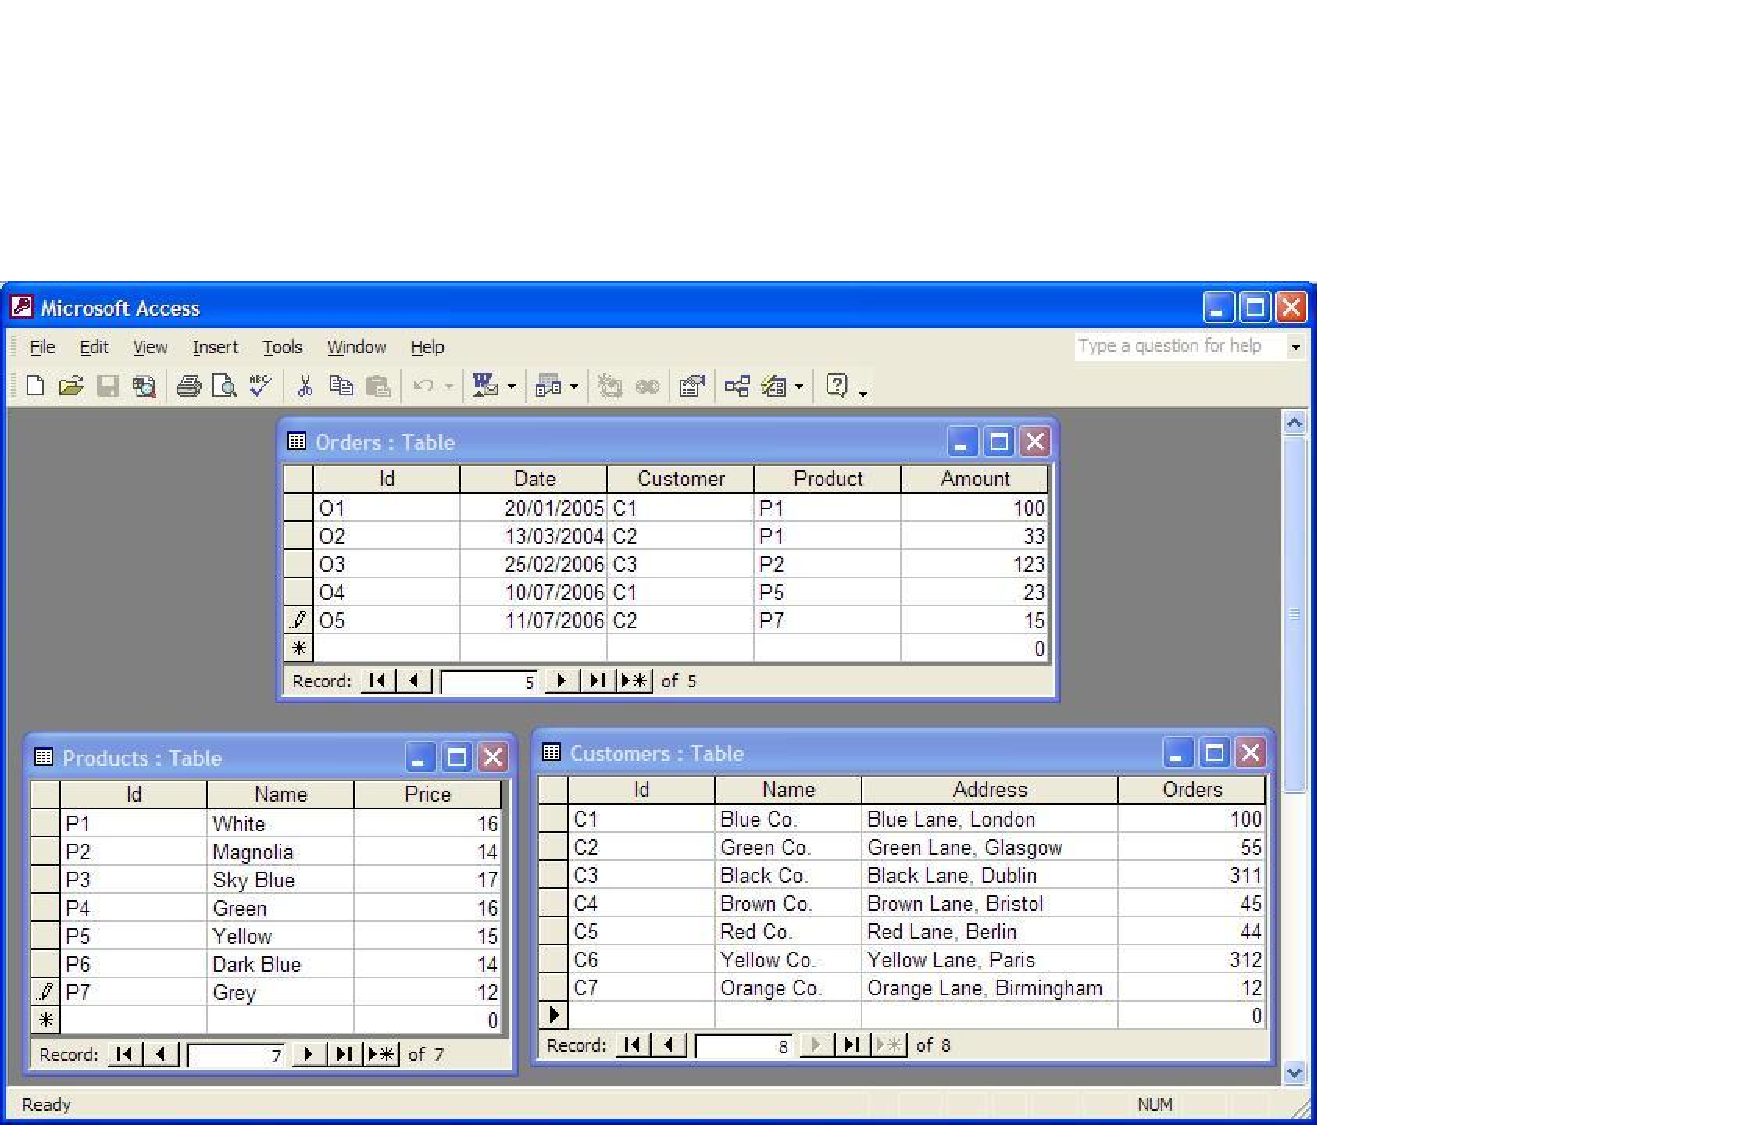
\includegraphics[width=12cm]{LanguageEngineering/Comprehensions/Images/Tables}

\caption{\label{fig:A-Customer-Order}A Customer Order Database}

\end{center}
\end{figure}


A typical example of data collections occurs in a relational database.
Figure \ref{fig:A-Customer-Order} shows a portion of a MS Access
database containing three tables relating to a pain manufacuring company.
The Customers table shows all the customers who have bought paint
from the company; each customer has a unique id, a name, an address
and a running tally of the number of orders that have ben placed.

The Products table shows all the types of paint that the company sells
along with the current price per unit. Finally, the Orders table shows
the orders that have been placed, linking customers, products and
amount.

Database tables contain records expressed as rows. Each table is modelled
as a class and the records modelled as instances of the class grouped
together as a set. The diagam in figure \ref{fig:Database-Tables-as}
shows three classes corresponding to the three database tables above.

%
\begin{figure}
\begin{center}

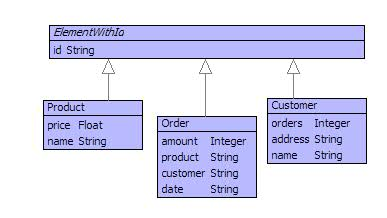
\includegraphics[width=12cm]{LanguageEngineering/Comprehensions/Images/Paint}

\caption{Database Tables as Classes\label{fig:Database-Tables-as}}

\end{center}
\end{figure}


The model above has chosen to represent the database tables directly:
each table uses the id field as a primary key and each class has modelled
this directly. Unlike database records, objects have a unique identity,
so this is not strictly necessary. It is useful to retain the id field
to show how database style queries and operations are supported by
the collection language construct below.

The database records are modelled as instances of the classes as shown
below:

\begin{lstlisting}
Root::Customers := Set{
  Customer("C1","Blue Co.","Blue Lane, London",100),
  Customer("C2","Green Co.","Green Lane, Glasgow",55),
  Customer("C3","Black Co.","Black Lane, Dublin",311),
  Customer("C4","Brown Co.","Brown Lane, Bristol",45),
  Customer("C5","Red Co.","Red Lane, Berlin",44),
  Customer("C6","Yellow Co.","Yellow Lane, Paris",312),
  Customer("C7","Orange Co.","Orange Lane, Birmingham",122)
};
Root::Products := Set{
  Product("P1","White",16),
  Product("P2","Magnolia",14),
  Product("P3","Sky Blue",17),
  Product("P4","Green",16),
  Product("P5","Yellow",15),
  Product("P6","Dark Blue",14),
  Product("P7","Grey",12)
};
Root::Orders := Set{
  Order("O1","20/01/2005","C1","P1",100),
  Order("O2","13/03/2004","C2","P1",33),
  Order("O3","25/25/2006","C3","P2",123),
  Order("O4","10/07/2006","C1","P5",23),
  Order("O5","11/07/2006","C2","P7",15)
};
\end{lstlisting}Each table is modelled as a global variable whose value is a set of
objects. New records can be added by updating the variable:

\begin{lstlisting}
@Operation newId(E:Set(ElementWithId)):String
  let i = 0
  in @While (not E->isEmpty) and 
            (not E->exists(e | e.id = "X" + i)) do
       i := i + 1
     end;
     i
  end
end
@Operation addCustomer(name:String,address:String)
  let id = newId(Customers) then
      newCustomer = Customer(id,name,address,0)
  in Root::Customers := Customers->including(newCustomer)
  end
end
\end{lstlisting}The operation newId is defined to automatically calculate a new identifier
for a collection of elements. The addCustomer operation modifies the
collection of customers by adding a newly constucted customer. Removing
customers can be achieved by a similar update to the global variable.

A query on one or more database tables involves performing a test
on each of the records in the table and producing a new table as a
result. In the model, a table is represented as a collection of elements.
The new language construct Cmp (short for \textit{comprehension})
allows us to do a query as follows:

\begin{lstlisting}
(1) @Operation ordersGreaterThan(x:Integer):Seq(Customer)
(2)   @Cmp customer where
(3)     customer <- Customers,
(4)     ? customer.orders > x
      end
    end
\end{lstlisting}The operation ordersGreaterThan (1) takes an integer x and returns
a collection of customers. Line (2) introduces the query as a Cmp
expression that returns all those customers (2) where each customer
is an element of the Customers table (3) and for which the orders
of each customer are grater than x (4).

A Cmp expression has the following general form:

\begin{lstlisting}
@Cmp body where clauses end
\end{lstlisting}A clause is either a binding (name <- collection) or a filter (? test).
The Cmp expression performs each clause in turn. A binding selects
each element from the collection in turn and, for each selection,
evaluates the rest ot the Cmp expression. A filter evaluates the test
(referencing any names bound tfrom its left); if the test succeeds
then evluation proceeds, otherwise evaluation retuns to the last selction
and tried with another element.

Consider the definition of ordersGreaterThan again. Line (3) causes
each sucessive customer to be selected from the Customers table. Line
4 allows only those customers to proceed whose orders value passes
the test. Finally, a sequence is returned containing all those customers
(2) that get through the test.

The following is an example of a query that involves multiple binding
and filters:

\begin{lstlisting}
@Operation customersWhoBuy(product:String):Seq(String)
  @Cmp c.name where
    c <- Customers,
    o <- Orders,
    p <- Products,
    ? p.name = product,
    ? o.customer = c.id,
    ? o.product = p.id
  end
end
\end{lstlisting}The operation customersWhoBuy is supplied with the name of a product
and returns a sequence of customer names for those customers who have
bought the supplied product.

A typical operation that occurs in a database is a \textit{join} where
two different tables are joined on two fields with the same value.
The records that have been defined so far have ben instances of specific
classes. A join does not necessary produce a record with a meaningful
type (although it might); section \ref{sub:Simple-Records} defines
a language construct for representing arbitrary records. The following
expression performs a join on the three tables producing a new table
of records showing the amount of each product for each customer:

\begin{lstlisting}
@Cmp 
  @Record
    customerName = c.name,
    productName = p.name,
    amount = o.amount
  end
where
  c <- Customers,
  p <- Products,
  o <- Orders,
  ? o.customer = c.id,
  ? o.product = p.id 
end
\end{lstlisting}%
\begin{figure}
\begin{center}

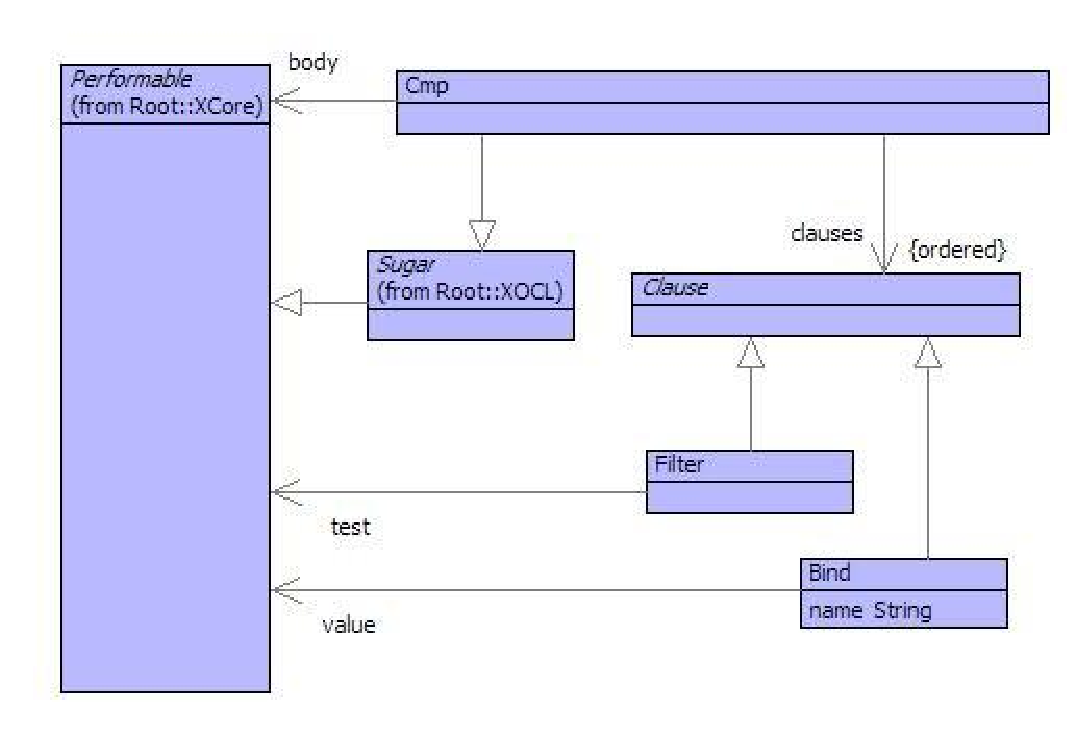
\includegraphics[width=12cm]{LanguageEngineering/Comprehensions/Images/Comprehensions}

\caption{Comprehensions\label{fig:Comprehensions}}

\end{center}
\end{figure}


A Cmp expression is defined in terms of a package of syntax classes
shown in figure \ref{fig:Comprehensions}. The class Cmp is defined
as sugar which means that it must define an operation called desugar
that turns an instance of Cmp into a Performable thing (usually an
instance of OCL classes). 

A Cmp has a performable body and a sequence of clauses. Each clause
is either a binding or a filer. A Cmp is desugared as follows:

\begin{lstlisting}
   @Operation desugar()
    @Case self of
(1)   Cmp(body,Seq{}) do
        [| Seq{<body>} |]
      end
(2)   Cmp(body,Seq{Bind(n,v)}) do
        [| <v> ->asSeq ->collect(<n> | <body>) |]
      end
(3)   Cmp(body,Seq{Bind(n,v)|clauses}) do
        [| <Cmp(Cmp(body,clauses),Seq{Bind(n,v)})>.flatten() |]
      end
(4)   Cmp(body,Seq{Filter(e)|clauses}) do
        [| if <e> then <Cmp(body,clauses)> else Seq{} end |]
      end
    end
  end
\end{lstlisting}The translation of a Cmp expression into basic XOCL is defined by
case analysis. Case (1) occurs when there are no clauses. In this
case the body is transformed into a single element sequence. Case
(2) occurs when there is a single binding. In this case the value
of the binding produces a collection and the body is performed for
each element of the collection producing a sequence. 

Case (3) occurs when there is a binding and some clauses. In this
case the following equivalence is used:

\begin{lstlisting}
@Cmp b where                            @Cmp 
  x <- S,         is equivalent to         @Cmp b where Cs end
  Cs                                    where
end                                       x <- S
                                        end->flatten
\end{lstlisting}Case (4) tests the expression e. If the result is true then the Cmp
expression proceeds otherwise it produces no elements. This has the
effect of filtering out the current variables that have been bound
so far.

Finally, the Cmp expression has a grammar that synthesizes an instance
of Cmp that, since it is an instance of Sugar, calls desugar automatically:

\begin{lstlisting}
@Grammar extends OCL::OCL.grammar
  Cmp ::= body = Exp cs = Clauses 'end' { Cmp(body,cs) }.
  Clauses ::= Where | { Seq{} }.
  Clause ::= Bind | Filter.
  Bind ::= n = Name '<-' e = Exp { Bind(n,e) }.
  Filter ::= '?' e = Exp { Filter(e) }.
  Where ::= 'where' c = Clause cs = (',' Clause)* { Seq{c|cs} }
end
\end{lstlisting}Applications for business intelligence and KPIs.


\section{Transforming Comprehensions}

The previous section has shown how a comprehension expression can
be transformed into an XOCL expression, thereby enriching XOCL with
a new language construct. Comprehensions have often been proposed
as a construct suitable for performing database queries since they
abstract away from the details of how the queries are performed and
how the result sets are built up.

A comprehension can be viewed as a query over a database if the tables
are viewed as sets of records. In this way the queries are performed
by selecting records, filtering them with predicates and joining them
back together. However, whilst this is an attractive way to construct
database queries, it does not solve the problems of how the queries
are performed and how the comprehensions can be embedded into a standard
programming language.

This section sketches out how comprehensions can be viewed as database
queries by showing how to desugar a comprehension into a standard
imperative language that provides a database interface. The translation
is deliberately simple; once it has been described the conclusion
outlines how the translation can be made more realistic.

Instead of the Cmp::desugar operation defined in the previous section,
a new operation is defined. The operation is called toSQL and takes
two arguments: the an expression to be transformed into an imperative
program and a variable. At run-time, the variable will be bound to
a set of values; after performing the comprehension program, the set
will contain the result. 

The toSQL operation proceeds by case analysis on the expression, each
case is addressed in turn. The first case deals with the aituation
where there are no qualifiers:

\begin{lstlisting}
@Operation toSQL(cmp,var)
  @Case cmp of
    Cmp(body,Seq{}) do
     [| let S = Set{}
        in <toSQL(body,[| S |])>;
           <var> := <var> ->including(S)
        end |]
    end
\end{lstlisting}The resulting program code creates a new set S and then uses this
as the container for the body of the comprehension. The resulting
set S is added to the supplied set (value of var). The next case deals
with a single filter:

\begin{lstlisting}
    Cmp(body,Seq{Filter(p)}) do
      [| if <p> 
         then <self.toSQL(Cmp(body,Seq{}),var)>
         else <var> := <var> ->including(Set{}) 
         end |]
    end
\end{lstlisting}If the predicate expression p is true then the body of the comprehension
is performed with the supplied var as the target set. Otherwise the
empty set is added to the target var. The next case deals with the
situation where there are multiple qualifiers:

\begin{lstlisting}
    Cmp(body,Seq{q|qs}) do
      [| <self.toSQL(Cmp(Cmp(body,qs),Seq{q}),var)>;
         <var> := <var> ->flatten;
         <var>
      |]
    end
\end{lstlisting}The same transformation as before is applied to the comprehension
whereby the multiple qualifiers are reduces by nesting the comprehension.
In this case the transformation on the nested comprehension will produce
an impreative program that updates the supplied set. Therefore, after
the supplied set is updated it is flattened before returning it. Finally,
the case where variables are bound is dealt with as follows:

\begin{lstlisting}
    Cmp(body,Seq{Bind(name,OCL::Var(tableName))}) do
      [| let S = DB.SQL("SELECT * FROM " + <tableName.lift()>);
             P = Set{}
         in @For <name> in S do
              <self.toSQL(body,[| P |])>
            end;
            <var> := <var> ->including(P)
         end |]
    end
  end
end
\end{lstlisting}Here it is assumed that all bindings select their elements from named
database tables. In this case the result set S is constructed by calling
a builtin procedure DB.SQL that takes an SQL query as a string. A
for-loop is used to iterate through the result set and the body of
the loop is generated by translating the body of the comprehension.
Notice that the set supplied to the body translation is P - the new
set created as part of the binding. The final action is to add the
set P to the supplied set var.

\begin{lstlisting}
let S = DB.SQL("SELECT * FROM " + "V");
    P = Set{}
in @For x in S do
     let S = DB.SQL("SELECT * FROM " + "W");
         P = Set{}
     in @For y in S do
          if x < y
          then
            let S = Set{}
            in S := S->including(x);
               P := P->including(S)
            end
          else
            P := P->including(Set{})
          end
        end;
        P := P->including(P)
     end;
     P := P->flatten
   end;
   S := S->including(P)
end;
S := S->flatten
\end{lstlisting}
